\documentclass[a4paper]{article}
\usepackage[utf8]{inputenc}
\usepackage[T1]{fontenc}

\usepackage[backend=biber,sorting=none]{biblatex}
\addbibresource{references.bib}

\usepackage{amsmath}
\usepackage{graphicx}
\usepackage{hyperref}
\usepackage{markdown}
\usepackage{placeins}

\title{FYS2085 project work: planetary motion}
\author{Mika Mäki}

\begin{document}
\maketitle
\tableofcontents

\section*{Introduction}
Newtonian gravity simulations are a cornerstone of modern astrophysics.
They can be used to model various astrophysical systems spanning several orders of magnitude all the way from an individual solar system to the merging of galaxies.

This project work provides an introduction to such n-body simulations by modeling the Solar System and investingating the effects of different simulation parameters on the results.

As a side note they can also be
\href{https://www.kerbalspaceprogram.com/}{highly entertaining} and beautiful to watch.

\href{https://beltoforion.de/en/spiral_galaxy_renderer/}{Approximations}


\clearpage
\section{Methods}
The n-body simulator of this project is based on the
\href{https://en.wikipedia.org/wiki/Verlet_integration#Velocity_Verlet}{velocity Verlet} integration algorithm.
Therefore its mathematical basis starts from the familiar Newton's second law
\begin{equation}
\overrightarrow{F} = m \overrightarrow{a},
\end{equation}
which relates the force $F$ to the resulting acceleration $a$ and the mass of the object $m$.
Using it the acceleration caused by the net effect of multiple forces is
\begin{equation}
\overrightarrow{a} = \frac{1}{m} \sum \overrightarrow{F_i}.
\end{equation}
Now if we approximate the acceleration to be constant over the time step of interest we have for the velocity and position
\begin{align}
v &= v_i + a_i \Delta t, \\
x &= x_i + v_i \Delta t + \frac{1}{2} a \Delta t^2.
\end{align}
Since these equations are highly prone to divergence due to slight numerical errors, adjustments are needed for better results.
This can be accomplished by averaging the accelerations of the current and previous timesteps, leading us to the Velocity Verlet algorithm
\begin{align}
x_{i+1} &= x_i + v_i \Delta t + \frac{1}{2} a_i \Delta t^2, \\
a_{i+1} &= \frac{F(x_{i+1})}{m}, \\
v_{i+1} &= v_i + \frac{1}{2}(a_i + a_{i+1}) \Delta t.
\end{align}

As this is a Newtonian gravity simulation, the forces between the objects are governed by the
\href{https://en.wikipedia.org/wiki/Newton\%27s_law_of_universal_gravitation}{Newton's law of gravitation}
\begin{equation}
F = G \frac{m_1 m_2}{r^2},
\end{equation}
where $G$ is the gravitational constant, $m_1$ and $m_2$ are the masses of the objects and $r$ is the distance between them.


\clearpage
\section{Implementation}
The program consists of two parts.
Fortran is used for the computation, and Python for the configuration of the simulation and plotting.
The interface between Fortran and Python is facilitated by
\href{https://numpy.org/doc/stable/f2py/}{F2PY} library, which is nowadays a part of
\href{https://numpy.org/}{Numpy}.
This program also uses several other libraries for plotting.
\href{https://matplotlib.org/}{Matplotlib} is used for exporting static images, and 
\href{https://www.pyqtgraph.org/}{PyQtGraph} is used for 3D graphics and animations.
PyQtGraph in turn is built upon the
\href{https://pypi.org/project/PySide6/}{PySide6} Qt bindings,
and also uses
\href{https://pypi.org/project/PyOpenGL/}{PyOpenGL} and
\href{https://pypi.org/project/PyOpenGL-accelerate/}{PyOpenGL-accelerate} to improve the performance of its 3D graphics.

The program is used through a Python file that contains the specification of the celestial bodies and the selection of tools to analyze the simulation with.
The \texttt{main.py} serves this purpose in this project.
The file \texttt{sim.py} contains the actual simulation wrapper that interacts with the Fortran-based simulation \texttt{core.f90}.

The \texttt{core.f90} Fortran module consists of the primary simulation loop \texttt{iterate} and the function \texttt{force} that it uses to compute the forces excerted on an object by the other celestial bodies.
It also contains some printing functions for arrays.
In addition to the Python bindings this module can be called from the Fortran main program \texttt{main.f90}.
This main program utilizes also the modules \texttt{cmd\_line.f90} and \texttt{utils.f90} that provide various utility functions.

The Fortran-based main program can be configured by modifying the ini-like configuration file \texttt{config.txt} in the \texttt{run} folder and passing it as a command-line argument.
The Python-based main program in turn is configured by modifying the values directly within \texttt{main.py}.

Instructions for building and running the program are available in the readme files in the repository.
Copies of those files are included here for convenience in appendix \ref{readmes}.




\clearpage
\section{Results}
Please see the attached code for interactive 3D visualizations.

\begin{figure}[ht!]
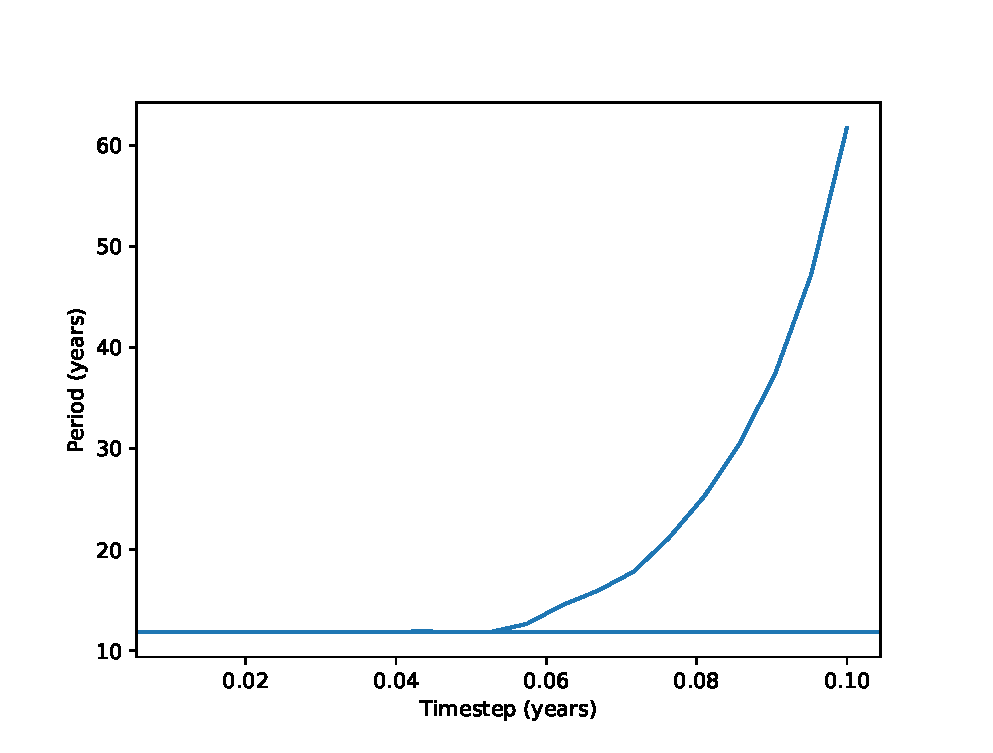
\includegraphics[width=\textwidth]{fig_1a.eps}
\caption{Period of Jupiter's orbit as a function of the simulation timestep (Part 1a)}
\end{figure}

For part 1b the motion of Jupiter was simulated for one orbital period, which was calculated from the radius and velocity of its orbit.
For a simulation timestep of 0.0395 years the rotation during the period was 0.864 degrees too small.


\FloatBarrier
\section{Conclusions}
The simulation works, but there is quite a bit of potential for optimization and further analysis.
It would be fascinating to run the code with a significant number of celestial bodies to model for example a galaxy.

Finally, sorry for the slightly late submission.
I've been doing over 45 credits this semester, so the past few weeks have been very busy.
In case the delay would affect the grade, could I perhaps do
some extra work during the Christmas holiday or submit an improved version of this project
when the course is lectured next year?
(It should be noted that despite the long period available for the project, I was able to start doing it only
a few days ago due to all other coursework, exams and the
\href{https://www.plancks.uk/london2020}{PLANCKS physics competition},
\href{https://github.com/AgenttiX/planetary-motion/commits/main}{as can be seen in the repository changelog},
and I miscalculated the time it took to get all the bugs ironed out.
)

\appendix
\clearpage
\section{Readme files}
\label{readmes}
\subsection{Build and install instructions}
\markdownInput{../src/README.md}

\clearpage
\subsection{Run instructions}
\markdownInput{../run/README.md}

\end{document}
